%%This is a very basic article template.
%%There is just one section and two subsections.
\documentclass[12pt, twoside]{article}
\usepackage[francais]{babel}
\usepackage[T1]{fontenc}
\usepackage[latin1]{inputenc}
\usepackage[left=6mm, right=6mm, top=6mm, bottom=6mm]{geometry}
\usepackage{float}
\usepackage{graphicx}
\usepackage{array}
\usepackage{multirow}
\usepackage{amsmath,amssymb,mathrsfs}
\usepackage{textcomp}
\usepackage{soul}

\pagestyle{empty}
\begin{document}

\begin{flushright}
$6^{eme}D$
\end{flushright}

\begin{flushleft}
Nom : \\
Prenom : 
\end{flushleft}
\section*{\center{Devoir maison}}


\textit{Le devoir Maison est  � rendre le \ul{Mardi 9 D�cembre 2008}. Les
exercices 1 et 3 sont � faire sur la photocopie (n'oubliez pas de marquer votre
nom). Les exercices 2 et 4 sont � faire sur votre copie double.}

\subsection*{Exercice 1}
\begin{center}
	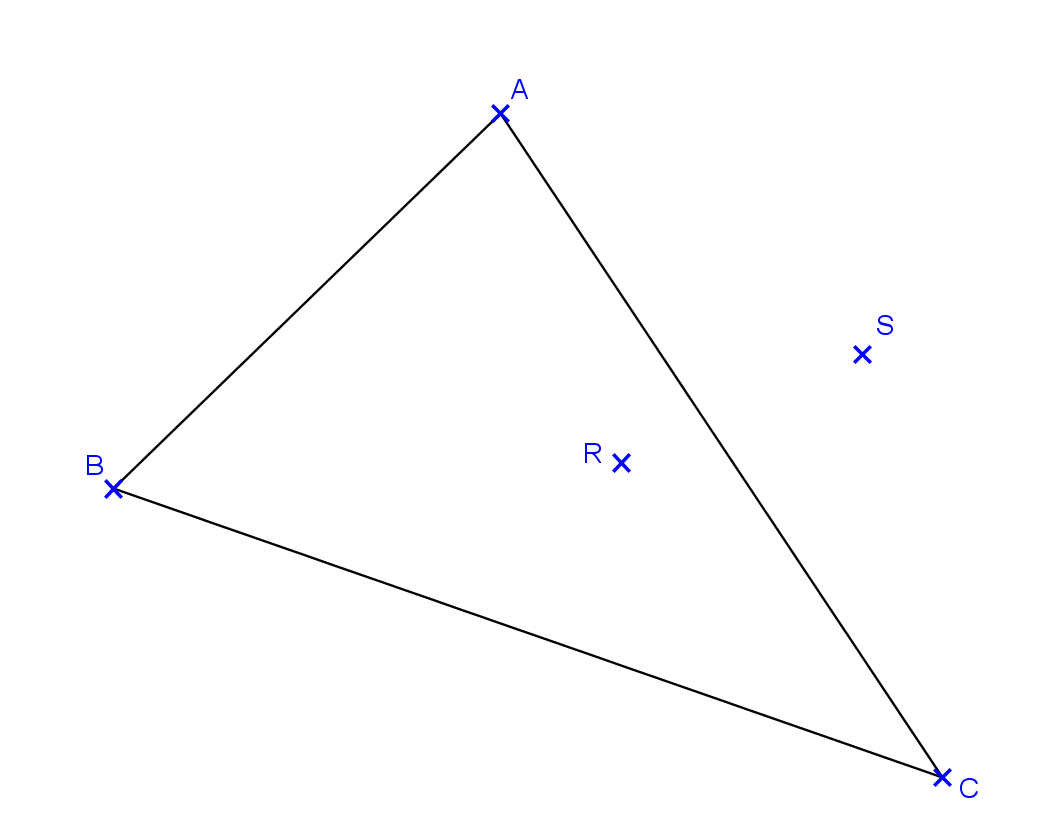
\includegraphics[width=14cm]{images/exo1.png}
\end{center}

Sur la figure ci-dessus, tracer � l'aide d'une �querre et (ou) d'une r�gle gradu�e : 
\begin{enumerate}
  \item en bleu la parall�le � la droite $(AB)$ passant par le point $R$,
  \item en rouge la perpendiculaire � la droite $(AC)$ passant par le point $R$,
  \item en vert la parall�le � la droite $(BC)$ passant par le point $S$.
\end{enumerate} 
\bigskip


\subsection*{Exercice 2}
\begin{tabular}{ccc}
\begin{minipage}{8cm}
Tracer une figure (� l'aide d'une �querre et (ou) d'une r�gle gradu�e) respectant les codages et les informations
donn�es sur le sch�ma ci-contre.
\end{minipage}
&$\ \ \ \ $&
\begin{minipage}{7cm}
\begin{center}
	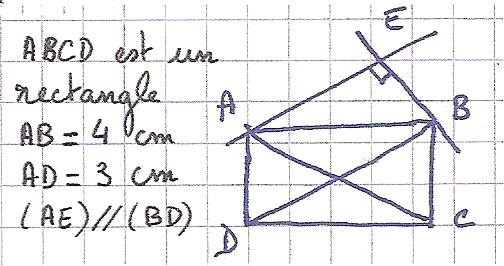
\includegraphics[width=7cm]{images/exo4.JPG}
\end{center}
\end{minipage}
\end{tabular}
\bigskip


\subsection*{Exercice 3}

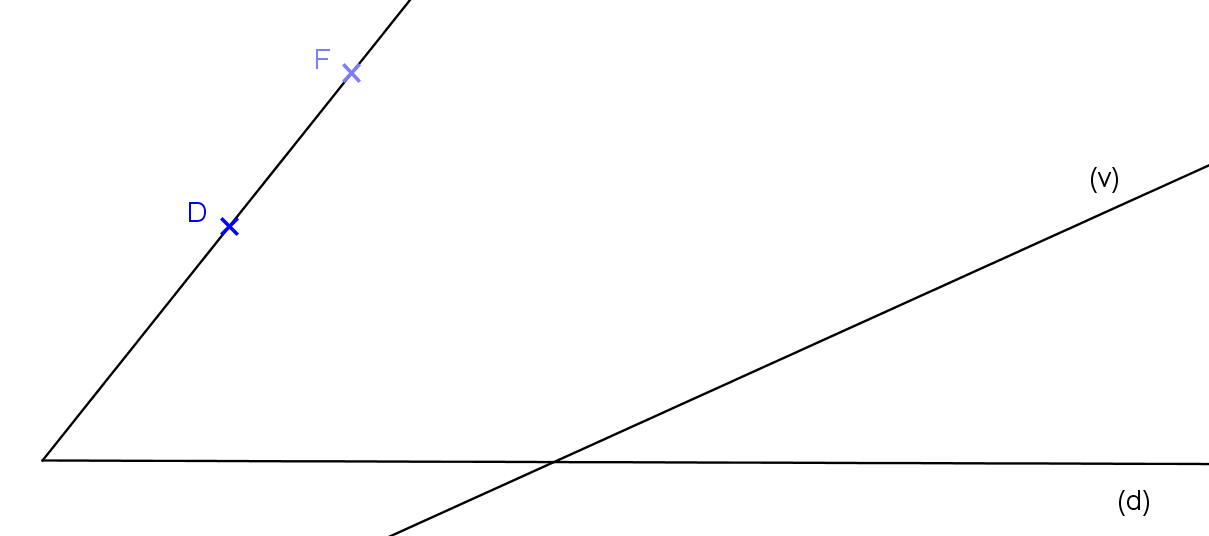
\includegraphics[width=14cm]{images/exo2.png}

\begin{enumerate}
  \item Tracer la perpendiculaire $(d_{1})$ � la droite $(v)$ passant
  par le point $D$.
  \item Tracer la perpendiculaire $(d_{2})$ � la droite $(v)$ passant
  par le point $F$.
  \item  Que peut-on dire des droites $(d_{1})$ et $(d_{2})$?
  
\rule{180mm}{0.5pt}


 \rule{180mm}{0.5pt} 
  \item Compl�ter la phrase: \textit{Les droites $(d_{1})$ et
  $(d_{2})$ sont \ldots \ldots \ldots \ldots \ldots \ldots \ldots parce
  qu'elles sont toutes les deux \ldots \ldots \ldots   \ldots \ldots \ldots \ldots � la droite (\ldots).}
  \item Citer la propri�t� du cours qui permet de l'affirmer?
  
  \rule{180mm}{0.5pt}
  
  \rule{180mm}{0.5pt}
  
  \rule{180mm}{0.5pt}
  
 \item Compl�ter:
 \begin{center}
 
\begin{tabular}{cc}
 \begin{minipage}{6cm}
 \ul{Donn�es}\\
 \ldots \ldots \ldots \ldots \ldots\\
 \ldots \ldots \ldots \ldots \ldots
 \end{minipage}       
&  
\begin{minipage}{6cm}
\ul{Conclusion}
\medskip

donc \ldots \ldots \ldots \ldots
\end{minipage}
 \end{tabular}
  \end{center}
  \end{enumerate}

\bigskip


\subsection*{Exercice 4}
Dans le quadrilat�re suivant, on sait qu'il y a 3 angles droits:

\center{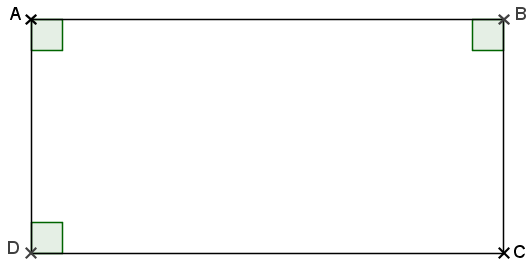
\includegraphics[width=6cm]{images/exo3.png}}

\begin{enumerate}
  \item \begin{enumerate}
          \item Recopier et compl�ter avec $//$ ou $\perp$:
          
         On sait que $(AD) \ldots (AB)$ et $(BC) \ldots (DC)$ alors $(AD)
         \ldots (BC)$.
         \item Citer la prorpri�t� du cours qui permet de l'affirmer.
\end{enumerate}

\item \begin{enumerate}
          \item Recopier et compl�ter avec $//$ ou $\perp$:
          
         On sait que $(AD) \ldots (BC)$ et $(AD) \ldots (DC)$ alors $(DC)
         \ldots (BC)$.
         \item Citer la prorpri�t� du cours qui permet de l'affirmer.
\end{enumerate}
\item Quelle est alors la figure obtenue?
\end{enumerate}

\end{document}
